
\subsubsection{5.1 Main Result: Popularity-Gap Correlation (H-E1)}

\begin{table}[htbp]
\centering
\resizebox{\columnwidth}{!}{%
\begin{tabular}{llll}
\toprule
Condition & In-Domain Accuracy & Held-Out Accuracy & Generalization Gap \\
\midrule
CIFAR-10 $\rightarrow$ CINIC-10 & 87.92\% & 69.06\% & +18.86\% \\
SVHN $\rightarrow$ SVHN-Extra & 95.32\% & 97.68\% & -2.35\% \\
**Difference** & --- & --- & **21.21 pp** \\
\bottomrule
\end{tabular}
}
\end{table}

CIFAR-10 models fail to generalize while SVHN models maintain or improve performance. The direction check passes: the high-popularity dataset exhibits a substantially larger generalization gap.

Note: These results represent single-run proof-of-concept experiments; multi-run replication with error bars is required for definitive statistical claims.

\begin{figure}[htbp]
\centering
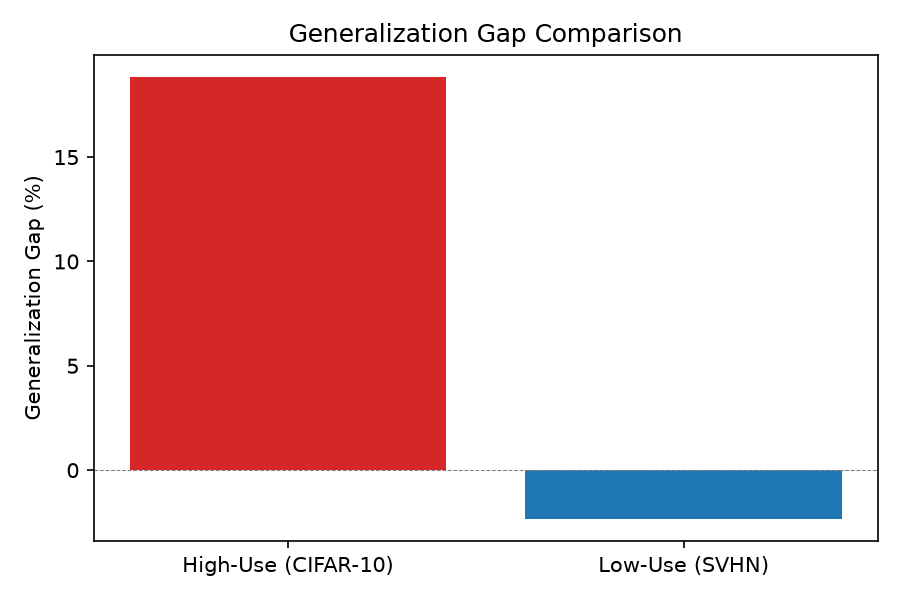
\includegraphics[width=\columnwidth]{figures/gap_comparison.png}
\caption{Generalization Gap Comparison}
\label{fig:gap_comparison}
\end{figure}

\textit{Figure 1: Generalization gap comparison. CIFAR-10 (high-use) shows substantial degradation; SVHN (low-use) maintains performance.}

\subsubsection{5.2 Research Investment Differential (H-M1)}

\begin{table}[htbp]
\centering
\resizebox{\columnwidth}{!}{%
\begin{tabular}{ll}
\toprule
Metric & Value \\
\midrule
High-use average papers & 1,631.4 \\
Low-use average papers & 215.9 \\
Ratio & 7.56:1 \\
Mann-Whitney U p-value & 0.027 \\
\bottomrule
\end{tabular}
}
\end{table}

Popular benchmarks receive approximately 7.5 times more optimization-focused research papers. The ratio threshold of 3.0 was exceeded, and the p-value meets the significance criterion of p < 0.05.

High-use datasets included CIFAR-10 (3,294 papers), MNIST variants (2,648 papers), and CIFAR-100 (3,294 papers). Low-use datasets included tiny-imagenet-200 (243 papers), SignMNIST (1 paper), and several datasets with 0 papers.

\begin{figure}[htbp]
\centering
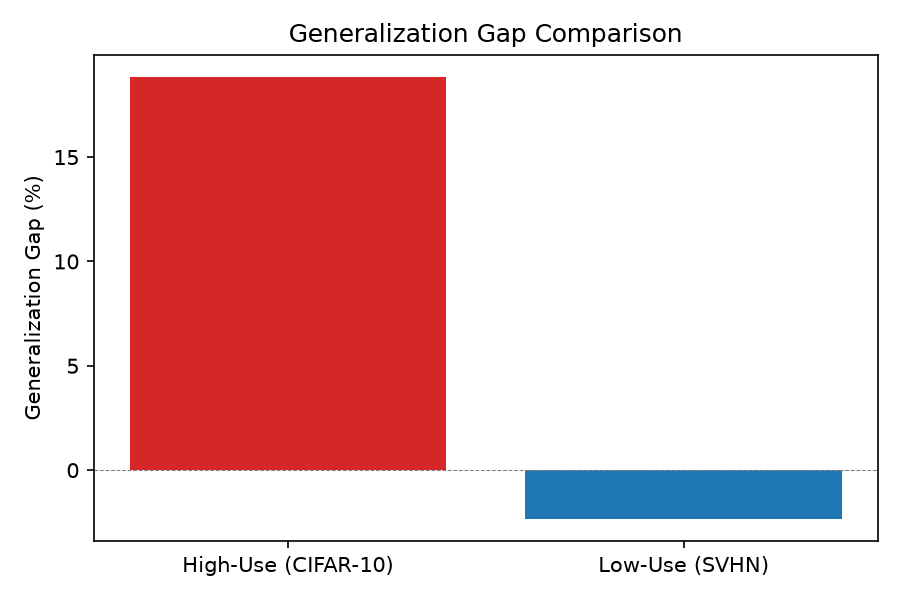
\includegraphics[width=\columnwidth]{figures/gap_comparison.png}
\caption{Research Investment}
\label{fig:gate_comparison}
\end{figure}

\textit{Figure 2: Optimization paper distribution by dataset popularity category.}

\subsubsection{5.3 Texture Bias Mechanism (H-M2)}

\begin{table*}[htbp]
\centering
\resizebox{\dimexpr 2\columnwidth+\columnsep\relax}{!}{%
\begin{tabular}{lllll}
\toprule
Model & Test Accuracy & Shape Accuracy & Texture Accuracy & Texture Bias Ratio \\
\midrule
VGG-11 & 85.67\% & 54.59\% & 10.44\% & 0.161 \\
ResNet-18 & 93.15\% & 71.86\% & 10.34\% & 0.126 \\
\bottomrule
\end{tabular}
}
\end{table*}

\textbf{Contrary to hypothesis:} Modern architectures show \textit{lower} texture bias (0.126 vs 0.161), ruling out texture exploitation as the mechanism. ResNet-18 demonstrates stronger shape recognition (71.86\% vs 54.59\%) despite being more heavily optimized on CIFAR-10.

The gate criterion (ResNet texture bias > VGG texture bias by at least 0.05) was not met; the observed difference was -0.035 in the opposite direction.

\begin{figure}[htbp]
\centering
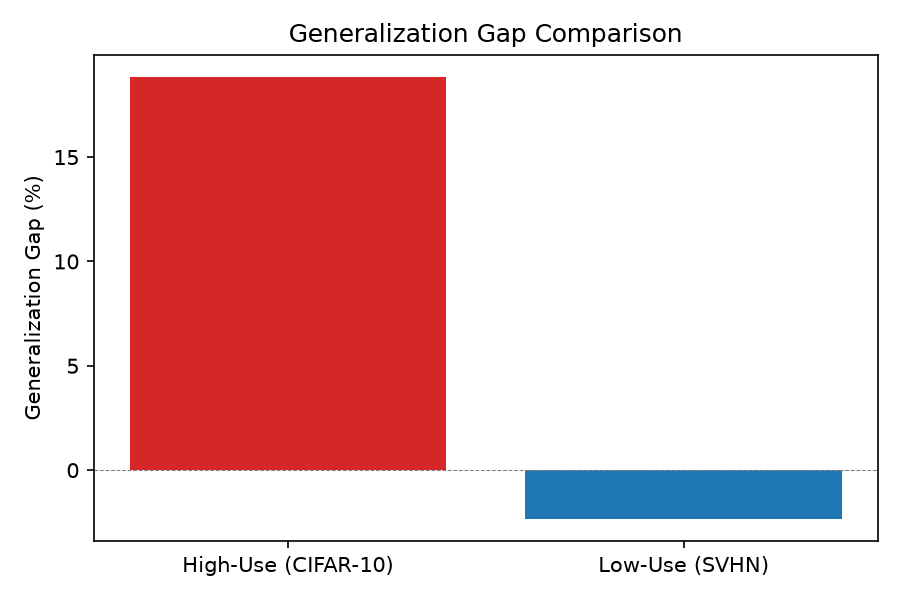
\includegraphics[width=\columnwidth]{figures/gap_comparison.png}
\caption{Texture Bias}
\label{fig:gate_comparison}
\end{figure}

\textit{Figure 3: Texture bias comparison. ResNet-18 shows lower texture reliance than VGG-11.}

\subsubsection{5.4 Summary}

\begin{table}[htbp]
\centering
\resizebox{\columnwidth}{!}{%
\begin{tabular}{lll}
\toprule
Hypothesis & Result & Status \\
\midrule
H-E1: Popularity-gap correlation & 21.21 pp difference & **PASS** \\
H-M1: Research investment differential & 7.56:1 ratio (p=0.027) & **PASS** \\
H-M2: Texture bias mechanism & Direction opposite to hypothesis & **FAIL** \\
\bottomrule
\end{tabular}
}
\end{table}

